\section{Dispositivos de expansi\'on}

Estos elementos realizan diversas funciones para el correcto funcionamiento del sistema, entre ellas tenemos:
\begin{itemize}
    \item Regulan la cantidad de fluido refrigerante que debe entrar en el evaporador
    \item Mantienen las presiones de alta y baja del circuito
    \item Producen la expansi\'on del fluido, para que \'este pase de alta a baja presi\'on
\end{itemize}

Pueden ser de varios tipos:
\begin{enumerate}[a.]
    \item Tubos capilares
    \item V\'alvulas de expansi\'on termost\'aticas
    \item V\'alvulas reguladoras de nivel (flotador)
    \item V\'alvulas manuales
\end{enumerate}

Las v\'alvulas manuales tienen muy poca aplicaci\'on. Son v\'alvulas de aguja y se emplean en instalaciones cuya carga sea constante. Tambi\'en se utilizan montadas en ``by-pass'' con las v\'alvulas de expansi\'on, como complemento de regulaci\'on, o bien para que en un momento dado, por ejemplo una aver\'ia, se pueda regular la cantidad de fluido a trav\'es de ellas.

\subsection{Tubos capilares}

Se las emplean en pequeñas instalaciones en las que var\'ia poco la carga frigor\'ifica, como instalaciones dom\'esticas, comerciales o acondicionamiento de aire.

\begin{figure}[H]
    \centering
    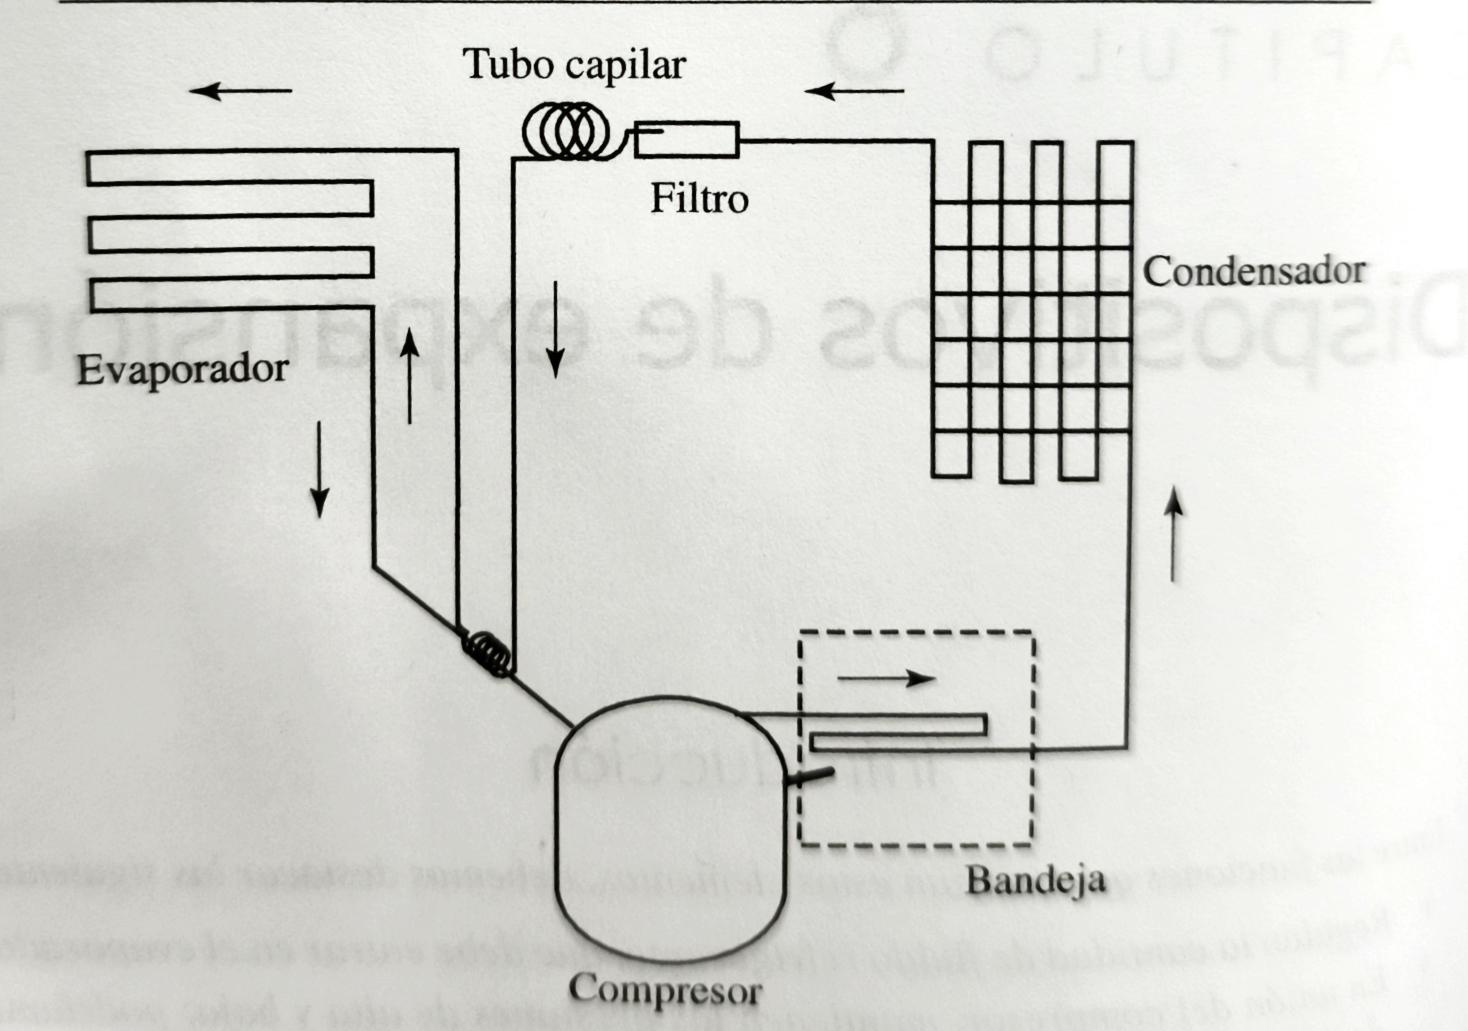
\includegraphics[width=0.6\linewidth]{figuras/dispositivos-de-expansion/circuito de heladera doméstica.jpg}
    \caption{Circuito de heladera dom\'estica}
    \label{fig:circuito-heladera-domestica}
\end{figure}

La l\'inea de trazos representa la bandeja de recogida de las gotas de agua resultantes de la condensaci\'on del aire en el interior de la heladera. En esta bandeja, al estar en contacto con el vapor recalentado de la descarga, se eliminan las gotas de agua. Asimismo, el fluido entra en el condensador con una temperatura menor, lo que favorece la condensaci\'on.

El tubo capilar une el condensador con el evaporador (alta y baja presi\'on), y es un tubo de cobre de pequeño di\'ametro. El fluido refrigerante al circular por el interior del tubo, sufre una ca\'ida de presi\'on y por lo tanto de temperatura, lo que origina su expansi\'on. Para evitar que una parte del fluido se evapore dentro del tubo, \'este se suele meter unos cent\'imetros dentro del tubo de aspiraci\'on (baja temperatura), que sale del evaporador hacia el compresor. Con lo que se produce un intercambio t\'ermico que retrasa la evaporaci\'on del fluido dentro del tubo capilar. 

Como se observa en \autoref{fig:circuito-heladera-domestica}, la instalaci\'on no lleva acumulador de l\'iquido, pues la reserva del fluido condensado se encuentra en los \'ultimos tramos del condensador, lo que a su vez hace de barrera entre el fluido condensado (hacia el tubo capilar) y la mezcla de l\'iquido y gas durante la condensaci\'on. En este tipo de instalaciones es muy importante la cantidad de refrigerante en el circuito para un correcto funcionamiento, en general ese dato lo facilitan los fabricantes.

\textbf{Las caracter\'isticas fundamentales de los tubos capilares son el di\'ametro interior y la longitud.} En caso de que estas no se respeten puede suceder que el fluido refrigerante pase con mayor rapidez al evaporador y \'este inundar\'ia, y llegar l\'iquido al compresor (longitud del tubo demasiado corta). O por el contrario (longitud del tubo demasiado larga), al fluido le costar\'ia llegar al evaporador, y el condensador se sebrecargar\'ia elevando su presi\'on y, con ello, disminuyendo la producci\'on frigor\'ifica.

\subsection{V\'avulas de expansi\'on termost\'aticas}

Esta v\'alvula es la encargada de expandir el refrigerante en estado l\'iquido para bajarle la presi\'on y temperatura, este l\'iquido puede venir subenfriado o no. A su vez, controla la cantidad de fluido refrigerante que va al evaporador, de esta manera, es capaz de mantener un recalentamiento constante para el \'optimo funcionamiento de la instalaci\'on. 

Deben montarse lo m\'as cerca posible de los evaporadores, pues de lo contrario, hay que compensar la p\'erdida de rendimiento, por ejemplo aislando el tramo que los une o cambiando di\'ametros de a cañería.

\textbf{Funcionamiento:}

Su funcionamiento queda determinado por tres presiones fundamentales que act\'uan sobre la membrana interior
\begin{figure}[H]
    \centering
    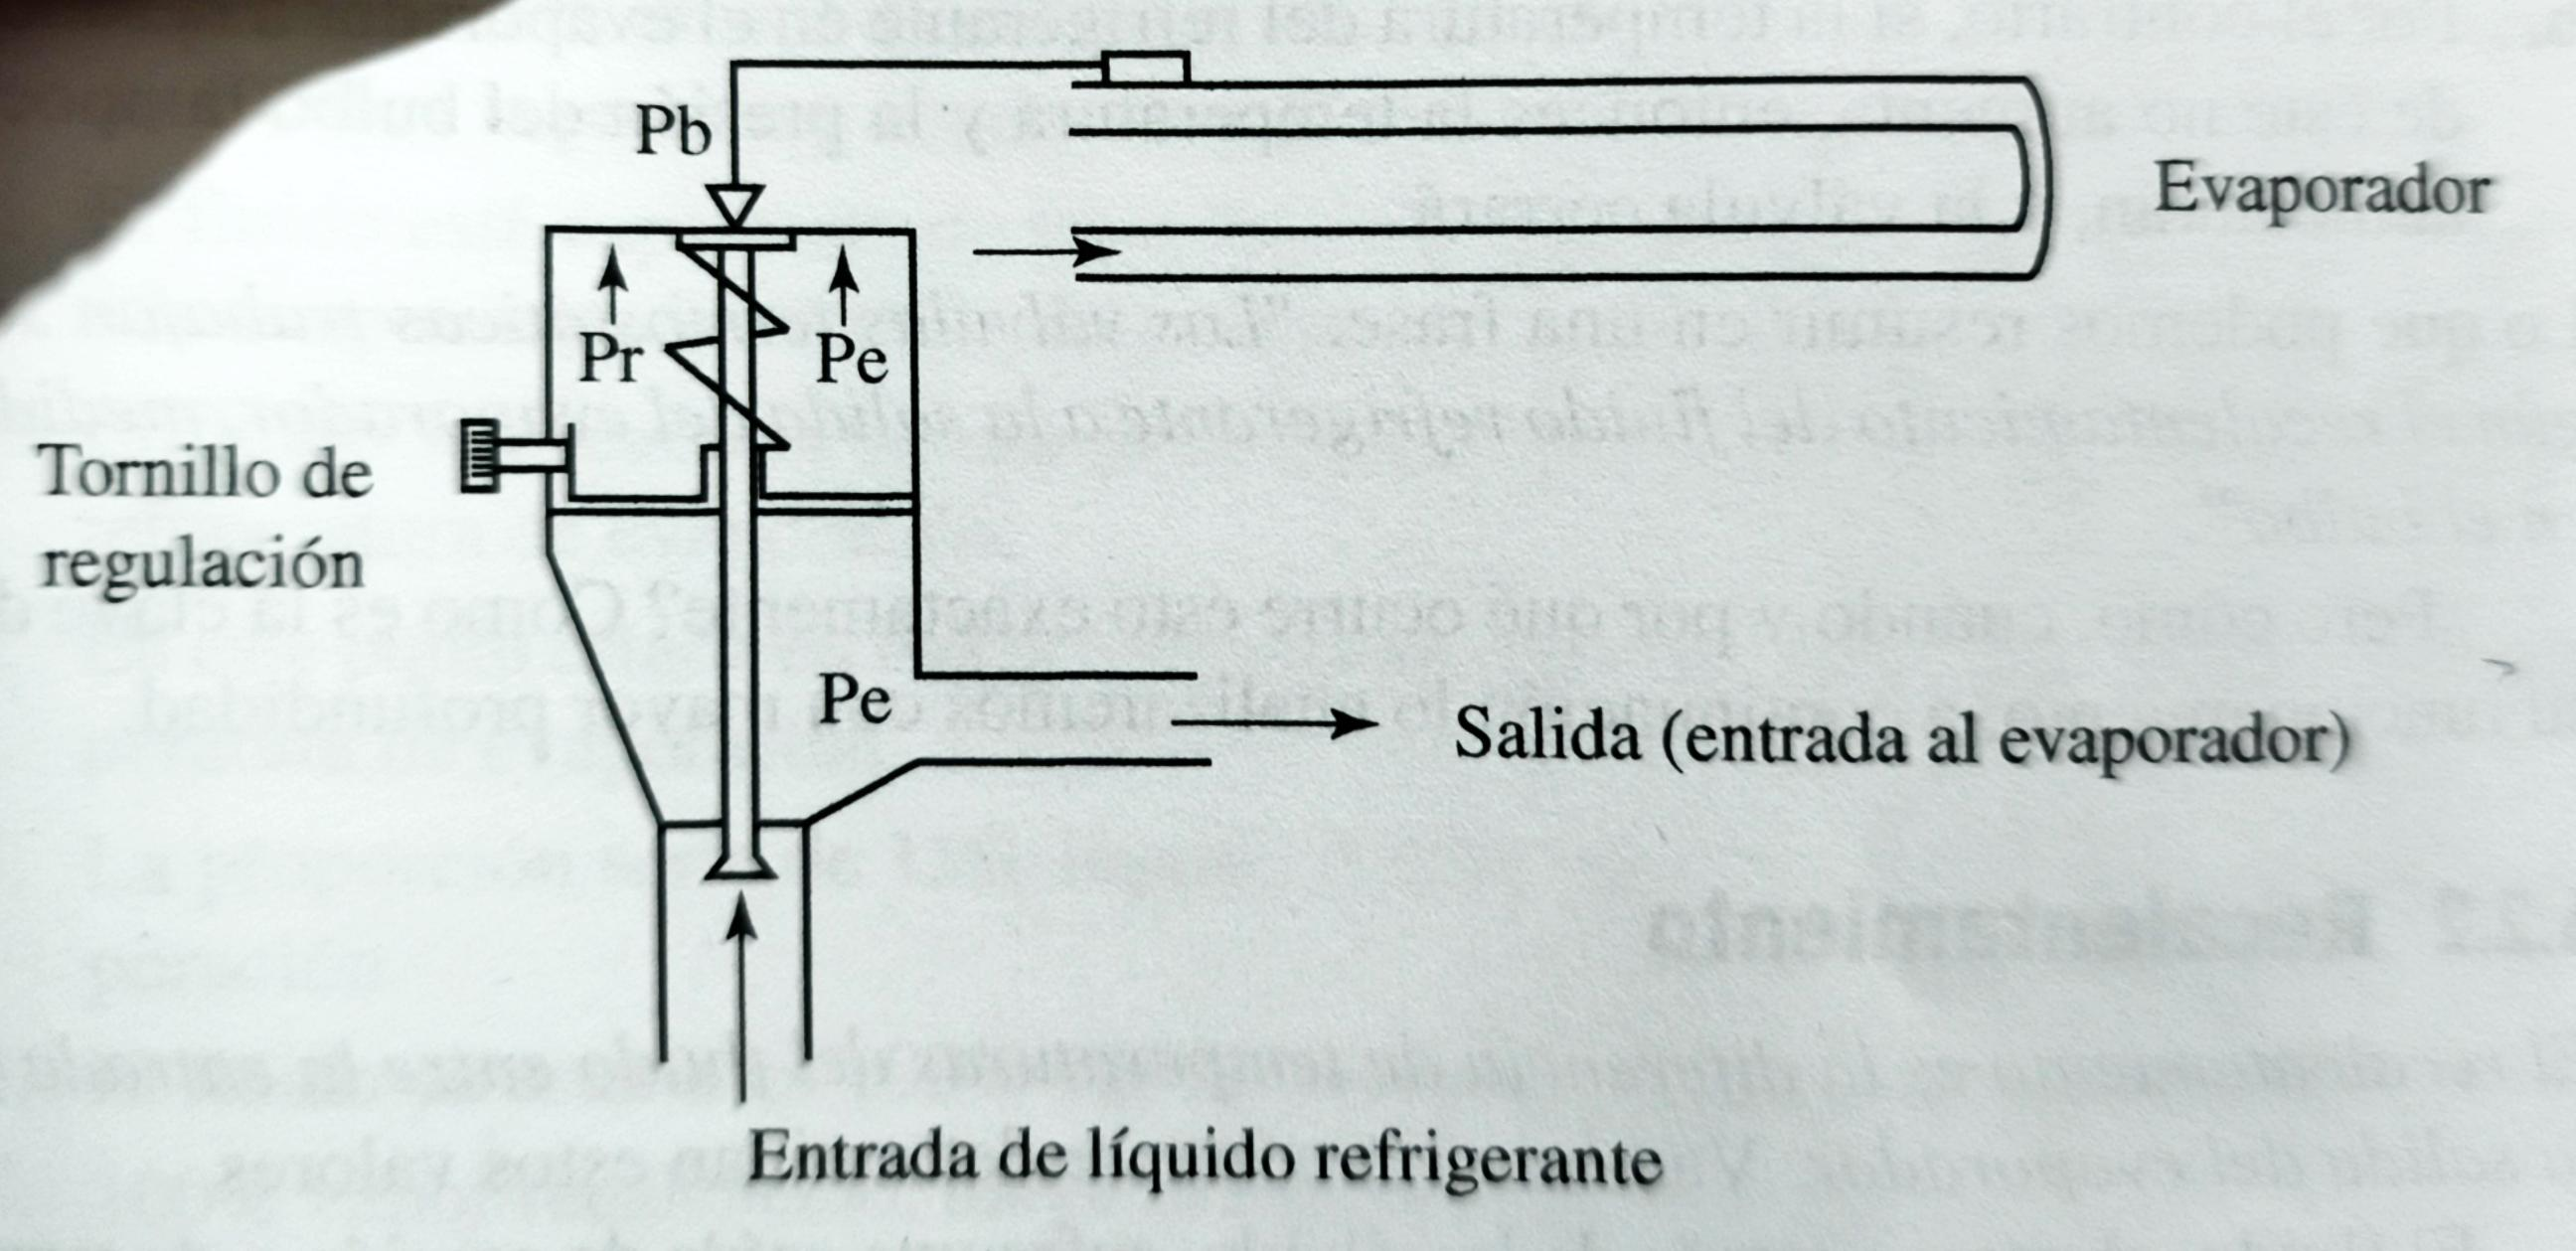
\includegraphics[width=.6\linewidth]{figuras/dispositivos-de-expansion/presiones-valvula-expansion.jpg}
    \caption{Presiones que act\'uan en v\'alvula de expansi\'on termost\'atica}
    \label{fig:presiones-valvula-termostatica}
\end{figure}

\begin{equation*}
    \frac{\downarrow Pb}{\uparrow Pr\ \uparrow Pe}
\end{equation*}

Por lo que, en su funcionamiento, la presi\'on del bulbo es equilibrada por la suma de la presi\'on del resorte m\'as la presi\'on de evaporaci\'on.

\begin{equation}
    Pb = Pr + Pe
    \label{eq:igualdad-presiones}
\end{equation}

donde

\begin{itemize}
    \item $Pb$ es la presi\'on del bulbo sobre la parte superior y tiende abrir la v\'alvula. El bulbo est\'a unido a la parte superior de la v\'alvula, mediante un tubo capilar soldado entre ambos
    \item $Pe$ es la presi\'on de evaporaci\'on, act\'ua sobre la parte inferior de la membrana y tiende a cerrarla
    \item $Pr$ es la presi\'on del resorte, tambi\'en act\'ua sobre la parte inferior de la membrana y tiende a cerrarla. Es la fuerza que act\'ua directamente sobre el v\'astago de la v\'alvula
\end{itemize}

\begin{gather*}
    \text{cuando}\ Pb > Pr + Pe \text{, la v\'alvula se abre}\\
    \text{cuando}\ Pb < Pr + Pe \text{, la v\'alvula se cierra}
\end{gather*}

La igualdad de presiones (\autoref{eq:igualdad-presiones}) se ver\'a afectada por la variaci\'on de la temperatura del refrigerante a la salida del evaporador medida en el bulbo ($Pb$), puesto que es la temperatura que act\'ua sobre el fluido que contiene el bulbo. S\'i, la temperatura aumenta a la salida del evaporador la $Pb$ aumenta y la v\'alvula se abrir\'a para dejar pasar m\'as fluido. En cambio, si disminuye la temperatura la v\'alvula se cerrar\'a restringiendo el paso del fluido.

Esto se puede entender con el recalentamiento del sistema. Se regula la v\'alvula termost\'atica mediante $Pr$, ante una variaci\'on de carga, la v\'alvula abrir\'a o cerrar\'a para mantener este recalentamiento constante. En general, el recalentamiento debe estar comprendido entre 4\textcelsius\ y 6\textcelsius. Para valores menores tendremos un bajo recalentamiento y en caso contrario, tendremos un alto recalentamiento.

\textbf{Recalentamiento bajo:}

En este caso, puede suceder que el llegue l\'iquido al compresor (si es muy bajo el recalentamiento) o que el compresor trabaje en r\'egimen h\'umedo, no llegandose a producir el golpe de l\'iquido. En ambos casos no es una situaci\'on favorable. Como un s\'intoma externo de la instalaci\'on se podr\'ia observar formaci\'on de escarcha o hielo en la culata del compresor.

Para corregir este inconveniente se procede a cerrar la v\'alvula, disminuyendo el caudal de refrigerante para lograr que \'este aumente su temperatura a la salida del evaporador.

\textbf{Recalentamiento alto:}

Esta situaci\'on supone una disminuci\'on en el rendimiento del evaporador, porque el refrigerante esta absorviendo calor sensible en vez de calor latente.

Como s\'intoma externo se podr\'ia observar un escarche parcial del evaporador, entendiendo que solo la parte escarchada estar\'ia funcionando como corresponde. Por otra parte, el compresor trabajar\'ia con ciclos largos a causa de la disminuci\'on de la superficie de transmisi\'on en el evaporador. Adem\'as, las temperaturas en la aspiraci\'on del mismo ser\'ian elevadas, lo que afectar\'ia en los materiales, lubricaci\'on y temperatura de descarga.

Como soluci\'on se deber\'ia desajustar la v\'alvula logrando dejar llegar mayor caudal de refrigerante al evaporador.

\textbf{Determinaci\'on del calentamiento:}

Con el presostato de baja presi\'on hallamos la presi\'on en el evaporador, con ella y utilizando el diagrama de mollier del refrigerante hallamos la temperatura de evaporaci\'on. Luego, con el term\'ometro colocado en el bulbo (salida del evaporador) hallamos la temperatura de salida del fluido, realizando la resta de estas temperaturas obtenemos el recalentamiento. 

\textbf{Circuito del bulbo:}

Es un circuito que contiene un fluido que puede estar en estado l\'iquido o gaseoso y este puede ser igual al de la instalaci\'on o no. Este fluido es el encargado de ir variando la apertura o cierre de la v\'alvula termost\'atica ($Pb$) cuando la temperatura a la salida del evaporador var\'ia. 

Los tiempos de respuesta de la v\'alvula seg\'un el estado del fluido que contiene el bulbo son:

\begin{table}[H]
    \centering
    \begin{tabular}{c c}\hline
    CARGA BULBO & TIEMPO RESPUESTA\\ \hline
    Vapor & Muy r\'apido\\
    L\'iquido & R\'apido\\
    Mezcla & Lento\\ \hline    
    \end{tabular}
\end{table}

\subsection{V\'alvula de expansi\'on termost\'atica con igualador externo de presi\'on}

En grandes evaporadores se produce una ca\'ida de presi\'on importante. Por tanto, s\'i se mide $Pe$ a la entrada del evaporador (como es en los casos de v\'alvulas con igualador interno), la temperatura de saturaci\'on que obtendr\'iamos con esa presi\'on no ser\'ia la verdadera. Por eso existen las v\'alvulas con igualador externo, estas toman la presi\'on del evaporador despu\'es del bulbo, es decir, tienen en cuenta la ca\'ida de presi\'on en el evaporador. Por tanto, la presi\'on para cerrar la v\'alvula es menor que si usar\'iamos una v\'alvula con igualador interno.

\textbf{Ejemplo de aplicaci\'on:}

En este caso tenemos una presi\'on de evaporador ($Pe$), que act\'ua para cerrar la v\'alvula es de $0,9 kg/cm^2$, que sumada a la presi\'on del resorte ($Pr$) cuyo valor es de $0.5 kg/cm^2$\ da una presi\'on total de cierre:

\begin{equation*}
    Pb = 0,5 + 0,9 = 1,4 kg/cm^2
\end{equation*}

que es la presi\'on necesaria en el bulbo para abrirla. Y tenemos una ca\'ida de presi\'on en el evaporador de $0,3 kg/cm^2$.

\begin{figure}[H]
    \centering
    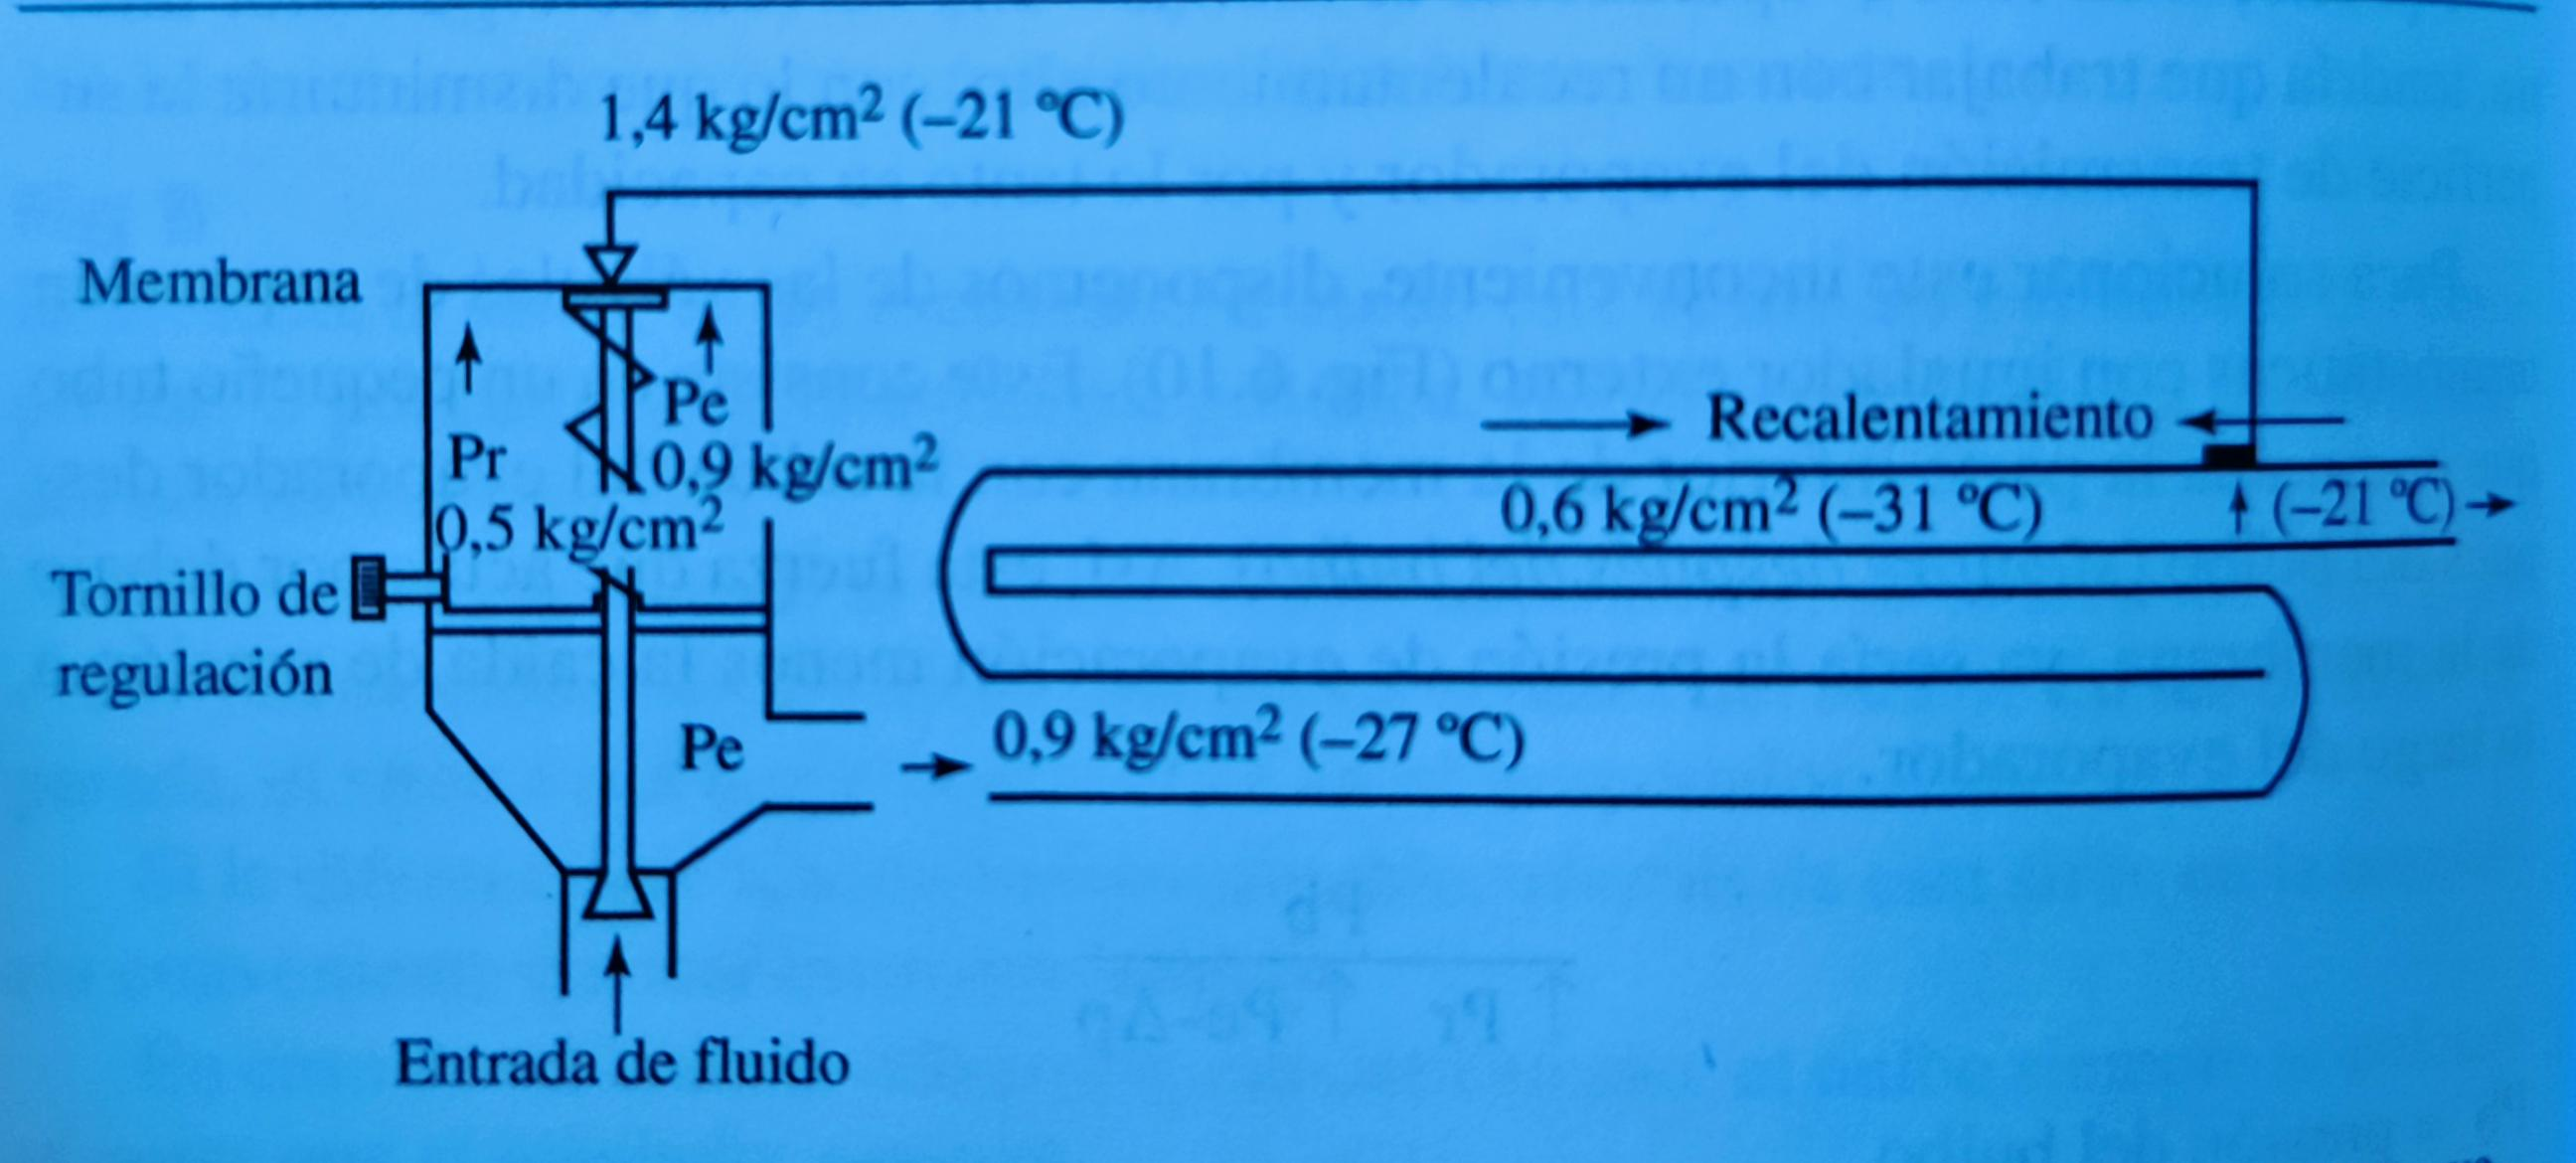
\includegraphics[width=0.6\linewidth]{figuras/dispositivos-de-expansion/funcionamiento-valvula-igualador-interno.jpg}
    \caption{Funcionamiento con v\'alvula de expansi\'on con igualador interno}
    \label{fig:valvula-igualador-interno}
\end{figure}

A esta presi\'on del bulbo le corresponde una temperatura de -21\textcelsius, por tanto la v\'alvula debe reducir el caudal de refrigerante para crear el recalentamiento necesario en el bulbo hasta alcanzar este valor. Dado que se produce una ca\'ida de presi\'on a lo largo del evaporador de $0,9 kg/cm^2$ a $0,6 kg/cm^2$, a esta presi\'on le corresponde una temperatura de -31\textcelsius, de esta manera, el recalentamiento es de 10\textcelsius. En consecuencia, \textbf{una excesiva ca\'ida de presi\'on en el evaporador con una v\'alvula de expansi\'on con igualador interno provoca un alto recalentamiento.}

Al utilizar una v\'alvula con igualador externo la presi\'on del evaporador tiene en cuenta la ca\'ida de presi\'on en \'el, lo que nos queda, $Pe = 0,6 kg/cm^2$. Esto se puede observar en la siguiente figura:

\begin{figure}[htbp]
    \centering
    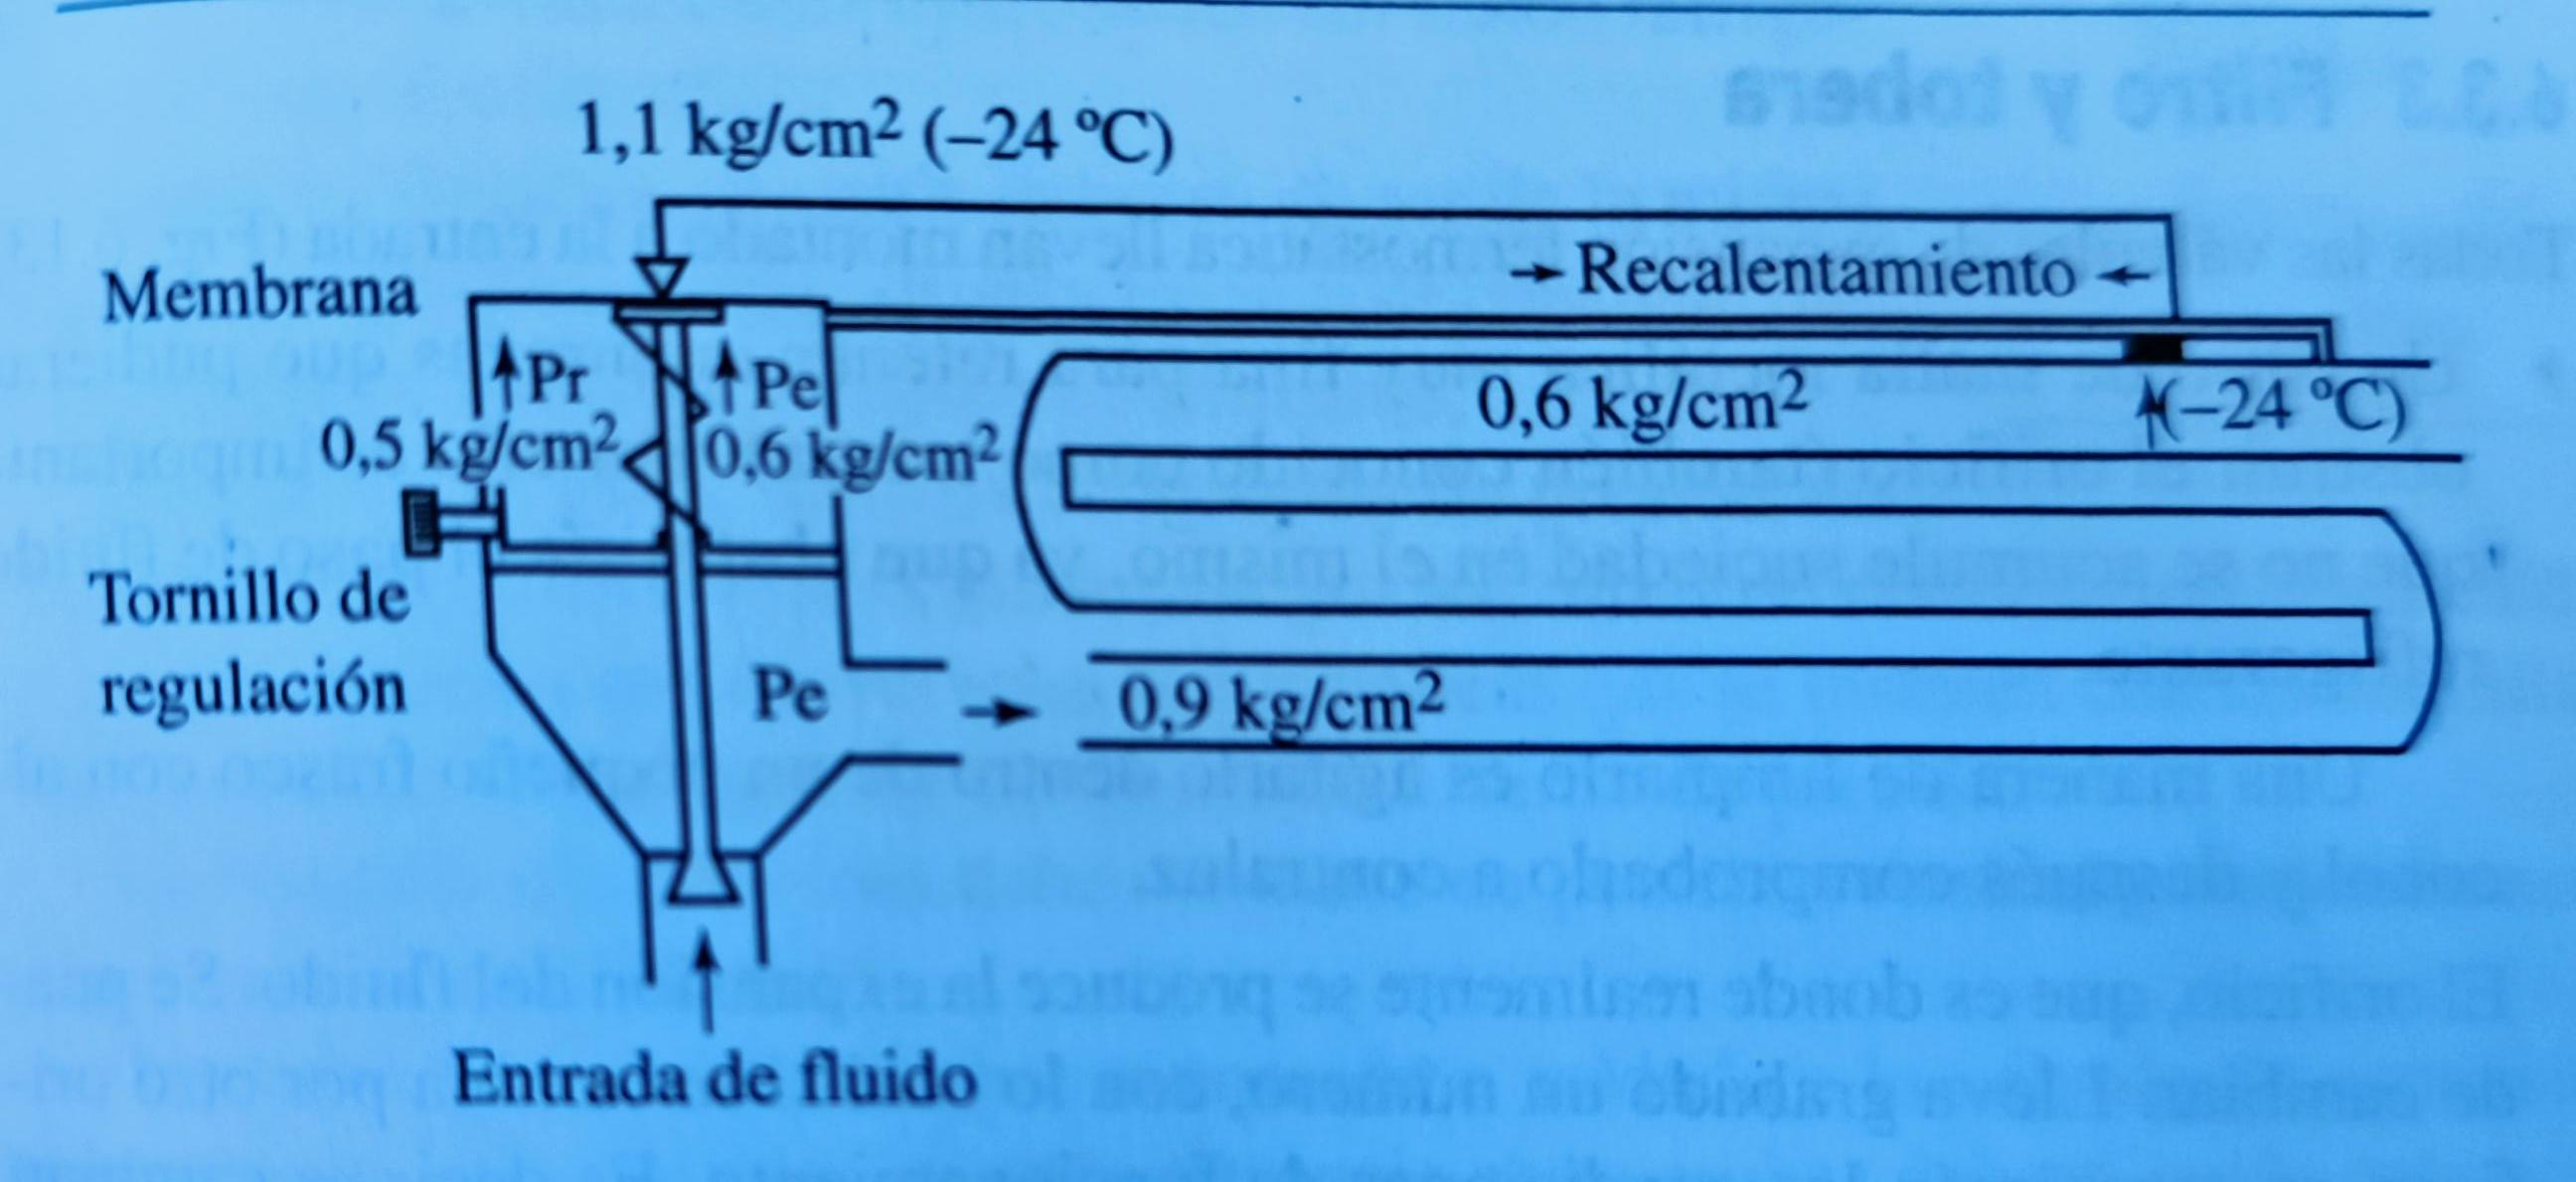
\includegraphics[width=.6\linewidth]{figuras/dispositivos-de-expansion/funcionamiento-valvula-igualador-externo.jpg}
    \caption{Funcionamiento con v\'alvula de expansi\'on con igualador externo}
    \label{fig:valvula-igualador-externo}
\end{figure}

Por tanto, la presi\'on de cierre nos queda:
\begin{equation*}
    Pb = 0,5 + 0,6 = 1,1 kg/cm^2
\end{equation*}

que a su vez es la presi\'on del bulbo necesaria para abrir la v\'alvula. A esta presi\'on del bulbo ($1,1 kg/cm^2$), le corresponde una temperatura de -24\textcelsius. A la presi\'on de salida del evaporador ($0,6 kg/cm^2$), le corresponde una temperatura -31\textcelsius, por lo que tenemos un recalentamiento de 7\textcelsius.

\subsection{V\'alvulas de expansi\'on termost\'aticas con MOP}

Son v\'alvulas limitadores de presi\'on. MOP es la presi\'on m\'axima de servicio. Es la presi\'on del evaporador a la cual la v\'alvula restringe el fluido refrigerante y evitan cualquier aumento de la presi\'on de aspiraci\'on del compresor.

Durante el ciclo de desescarche, y tambi\'en al finalizar, se produce un aumento de presi\'on en el evaporador, con lo que cuando el compresor volviera a ponerse en marcha, se encontrar\'ia con una presi\'on alta que sobrecargar\'ia el motor. Al instalar estas v\'alvulas evitamos que lo explicado anteriormente suceda.

Uno de los tipos m\'as empleados es el que tiene dos membranas y un elemento el\'astico entre ellas. Cuando la presi\'on de aspiraci\'on se aproxima al punto de sobrecarga del motor, el elemento el\'astico se comprime y obliga a la v\'alvula a restringir el paso de fluido refrigerante al evaporador. Entonces, la presi\'on de aspiraci\'on disminuye hasta la de ajuste, con lo cual el elemento el\'astico se extiende y las dos membranas act\'uan como una sola. A partir de ese momento la v\'alvula funciona de manera normal.

\begin{figure}[H]
    \centering
    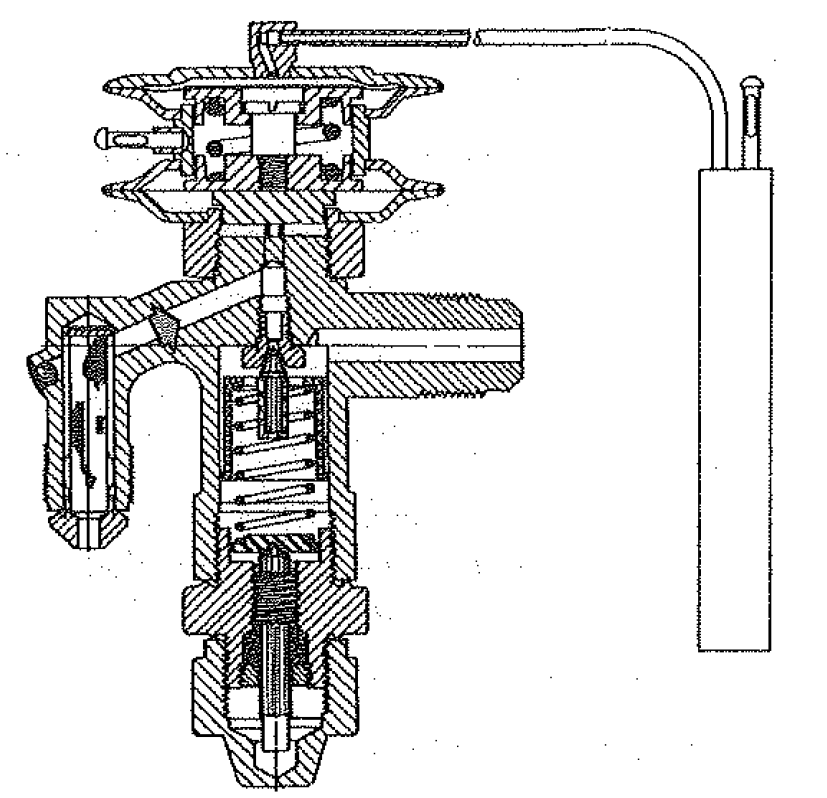
\includegraphics[width=.6\linewidth]{figuras/dispositivos-de-expansion/valvula-expansion-mop.png}
    \caption{V\'alvula de expansi\'on termost\'atica con MOP}
    \label{fig:valvula-expansion-mop}
\end{figure}

\subsection{Selección de la v\'alvula de expansi\'on termost\'atica}

La v\'alvula se selecciona a partir de los siguientes datos conocidos:

\begin{itemize}
    \item Capacidad de refrigeraci\'on
    \item Temperatura de evaporaci\'on
    \item Temperatura de condensaci\'on
    \item Tipo de refrigerante
    \item Ca\'ida de presi\'on neta a trav\'es de la v\'alvula (diferencia entre la presi\'on de alta y baja)
\end{itemize}

Con estos datos y las tablas de los fabricantes se seleccionan los dispositivos.

\subsection{V\'alvulas de expansi\'on de flotador}

Como se ha mencionado antes estas v\'alvulas se utilizan para alimentar los evaporadores de tipo ``inundados''.

El flotador se encarga de regular el nivel de l\'iquido refrigerante , actuando sobre una v\'alvula cuyo orificio de entrada es el que produce la expansi\'on del fluido. De hecho, si fuera necesario cambiar las condiciones del fluido (temperatura de expansi\'on m\'as baja), se podr\'ia realizar cambiando el tamaño del orificio. 

Estas v\'alvulas se clasifican en v\'alvulas de alta o baja presi\'on, seg\'un su posici\'on en la instalaci\'on, es decir en el lado de alta o baja presi\'on.

\subsubsection{V\'alvula de baja presi\'on}

Su misi\'on es mantener el nivel de l\'iquido en el evaporador, bien sea directamente sobre el evaporador o por medio del separador de l\'iquido, como se observa en la siguiente \autoref{fig:valvula-flotador-baja-presion}.

\begin{figure}[H]
    \centering
    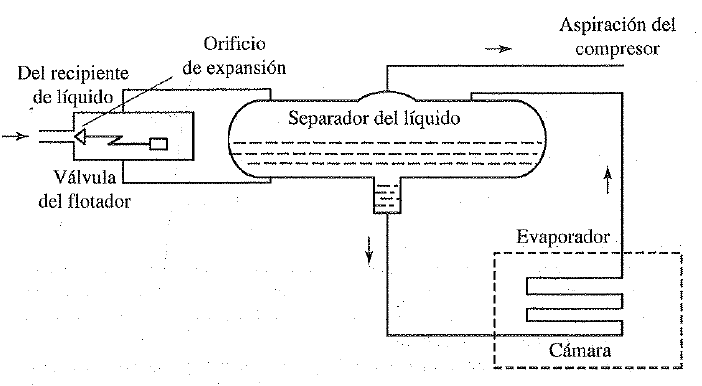
\includegraphics[width=.6\linewidth]{figuras/dispositivos-de-expansion/valvula-expansion-flotador.png}
    \caption{Instalaci\'on de la v\'alvula de baja presi\'on}
    \label{fig:valvula-flotador-baja-presion}
\end{figure}

La v\'alvula de flotador recibe el fluido en estado l\'iquido del recipiente. La expansi\'on se produce a trav\'es del orificio. Por lo tanto, la interpretaci\'on del funcionamiento es la siguiente:

\begin{itemize}
    \item A la entrada de la v\'alvula el fluido se encuentra en estado l\'iquido, procedente del recipiente.
    \item Sufre una expansi\'on, con lo cual en el interior de la envolvente de la v\'alvula, se encuentra en estado de gas y l\'iquido a baja presi\'on.
    \item Como el separador de l\'iquido es alimentado por la v\'alvula, se encuentratra en las mismas condiciones por ello est\'an perfectamente aislados.
    \item El evaporador es alimentado por fluido en estado l\'iquido a la misma temperatura que se expansion\'o
    \item Al bajar el nivel de l\'iquiod en el separador. seg\'un sea por la demanda del evaporador o bien por la aspiraci\'on del compresor, tambi\'en baja en el recipiente de la v\'alvula y el flotador abre dando entrada al fluido refrigerante, hasta que alcanza el nivel de regulaci\'on y cierra.
\end{itemize}

\subsubsection{V\'alvula de alta presi\'on}

Suele ir montada en el recipiente de l\'iquido. Cuando el nivel de l\'iquido en el recipiente sube, el flotador abre la v\'alvula y da paso de fluido expansionado al evaporador.

Por lo general se usan para alimentar evaporadores de carga constante, ya que al actuar en la alta presi\'on, dan paso de fluido independiente de la que realmente necesite el evaporador. Como en el caso de la v\'alvula de baja, al cambiar el orificio de la v\'alvula se cambian las condiciones de expansi\'on.

\begin{figure}[H]
    \centering
    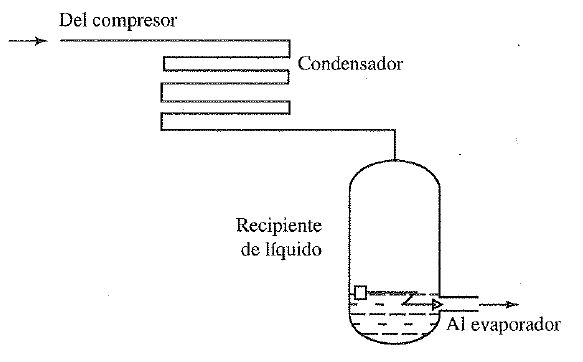
\includegraphics[width=.6\linewidth]{figuras/dispositivos-de-expansion/valvula-expansion-flotador-alta.png}
    \caption{Instalaci\'on de la v\'alvula de alta presi\'on}
    \label{valvula-flotador-alta-presion}
\end{figure}

\subsection{Subenfriamiento y sobrecalentamiento}

Midiendo los valores de subenfriamiento y sobrecalentamiento se puede saber como se esta comportando nuestro sistema. En la siguiente tabla se muestra los sintomas que puede tener el sistema seg\'un el valor del subenfriamiento y sobrecalentamiento.
\begin{table}[H]
    \centering
    \begin{tabular}{l c c} \hline
        Causa & Recalentamiento & Subenfriamiento\\ \hline
        Falta de refrigerante & Alto & Bajo\\
        Sobra refrigerante & Bajo & Alto\\
        Restricci\'on l\'inea de l\'iquido & Alto & Alto\\
        Exceso de l\'iquido en el evaporador & Bajo & Bajo\\ \hline
    \end{tabular}
\end{table}